\documentclass[11pt,letterpaper]{article}
\usepackage[T1]{fontenc}
\usepackage[utf8]{inputenc}
\usepackage{lmodern}
\usepackage[margin=0.9in]{geometry}
\usepackage{booktabs}
\usepackage{tabularx}
\usepackage{array}
\usepackage{float}
\usepackage{amsmath}
\usepackage[table]{xcolor}
\usepackage{enumitem}
\usepackage{caption}
\usepackage{tikz}
\usetikzlibrary{positioning,arrows.meta,shapes.geometric,fit,backgrounds,calc}
\usepackage[hidelinks]{hyperref}
\setlist{nosep,leftmargin=1.3em}
\captionsetup{font=small,labelfont=bf}
\newcolumntype{L}[1]{>{\raggedright\arraybackslash}p{#1}}

% ---------- diagram styles ----------
\tikzset{
  >={Stealth},
  box/.style={draw, rounded corners=3pt, align=center, font=\small, minimum height=9mm,
              text width=#1, inner sep=4pt},
  box/.default=34mm,
  data/.style={box=#1, fill=blue!10},
  proc/.style={box=#1, fill=gray!12},
  gate/.style={box=#1, fill=red!12, very thick},
  model/.style={box=#1, fill=green!12},
  out/.style={box=#1, fill=orange!18},
  rej/.style={box=#1, fill=white, dashed, text=gray!70!black},
  dec/.style={draw, diamond, aspect=2.2, fill=yellow!20, font=\small, align=center, inner sep=1pt},
  flow/.style={->, thick},
  side/.style={->, thick, dashed, gray},
  lab/.style={font=\scriptsize\itshape, text=gray!40!black}
}

\title{Question 7 Forecasting Pipeline: Flow and Components\\[2pt]
\large How data moves from raw food-shelf records to the August 2026 county submission}
\author{MinneMUDAC 2026 Undergraduate Team}
\date{Information cutoff: July 31, 2026}

\begin{document}
\maketitle
\sloppy

\noindent This document describes the \emph{structure} of the forecasting pipeline in
\texttt{forecast\_august\_2026/}: its stages, the scripts that implement them, what each one reads
and writes, where the information cutoff is enforced, and how the final model turns county history
into a forecast. The companion report (\texttt{forecasting\_report.pdf}) contains the results.

\section{End-to-end flow}

\begin{figure}[H]\centering
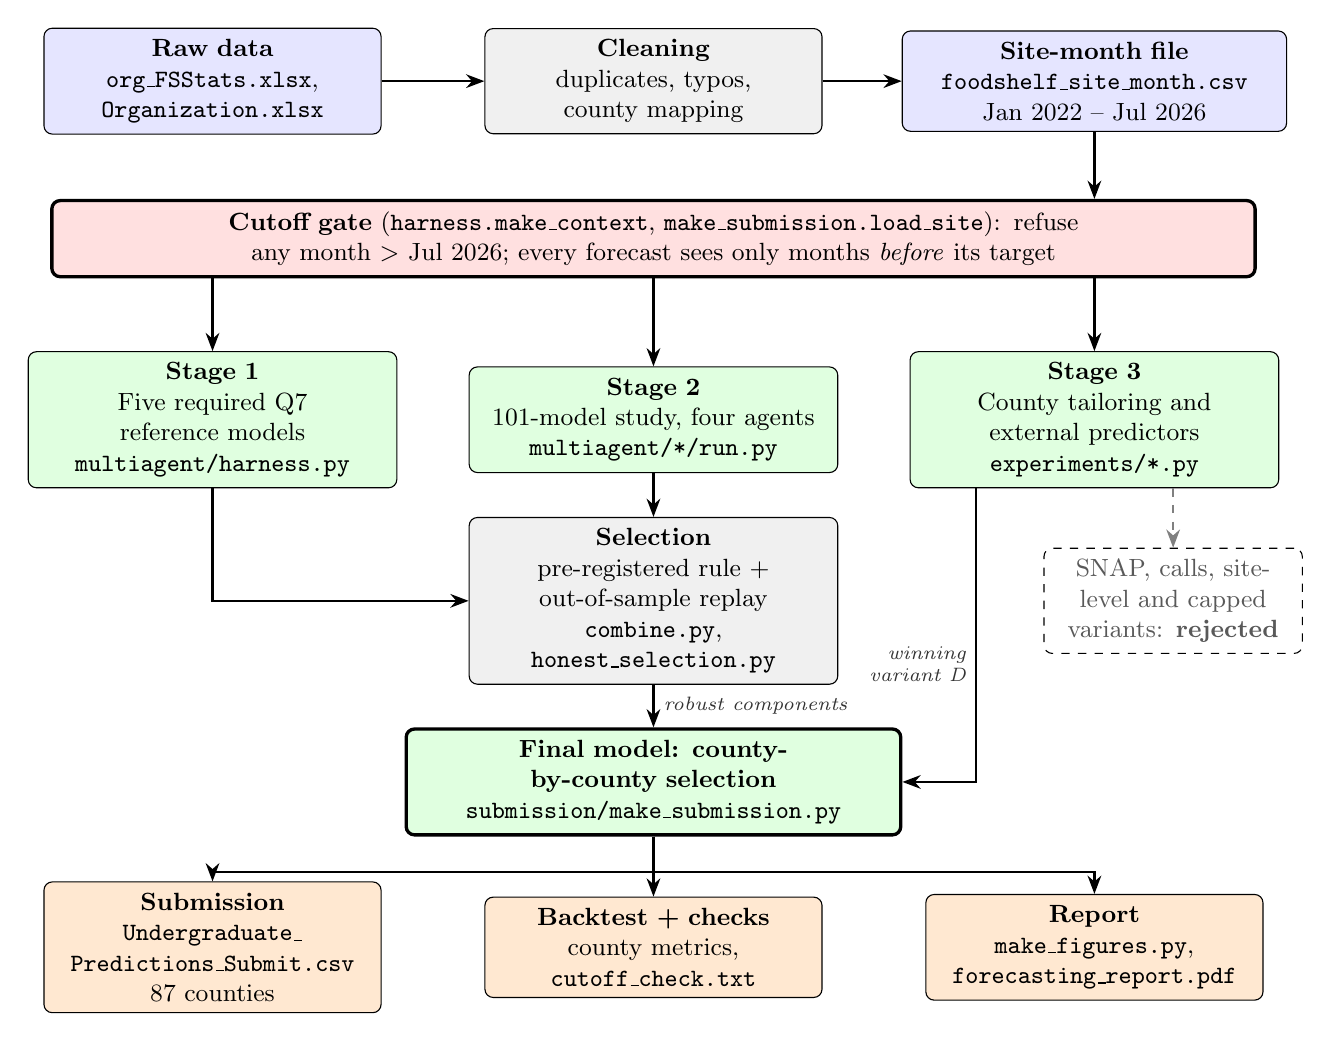
\begin{tikzpicture}[node distance=6mm]
% column x positions
\def\xa{0} \def\xb{5.6} \def\xc{11.2}
% row 1: data
\node[data=40mm] (raw) at (\xa,0) {\textbf{Raw data}\\ \texttt{org\_FSStats.xlsx}, \texttt{Organization.xlsx}};
\node[proc=40mm] (clean) at (\xb,0) {\textbf{Cleaning}\\ duplicates, typos, county mapping};
\node[data=46mm] (site) at (\xc,0) {\textbf{Site-month file}\\ \texttt{foodshelf\_site\_month.csv}\\ Jan 2022 -- Jul 2026};
\draw[flow] (raw) -- (clean);
\draw[flow] (clean) -- (site);
% row 2: gate
\node[gate=150mm] (gate) at (\xb,-2.0) {\textbf{Cutoff gate} (\texttt{harness.make\_context}, \texttt{make\_submission.load\_site}):
  refuse any month $>$ Jul 2026; every forecast sees only months \emph{before} its target};
\draw[flow] (site.south) -- ++(0,-0.5) -| (gate.north -| site);
% row 3: three stages
\node[model=44mm] (s1) at (\xa,-4.3) {\textbf{Stage 1}\\ Five required Q7 reference models\\ \texttt{multiagent/harness.py}};
\node[model=44mm] (s2) at (\xb,-4.3) {\textbf{Stage 2}\\ 101-model study, four agents\\ \texttt{multiagent/*/run.py}};
\node[model=44mm] (s3) at (\xc,-4.3) {\textbf{Stage 3}\\ County tailoring and external predictors\\ \texttt{experiments/*.py}};
\foreach \s in {s1,s2,s3} \draw[flow] (gate.south -| \s) -- (\s.north);
% row 4: selection
\node[proc=44mm] (sel1) at (\xb,-6.6) {\textbf{Selection}\\ pre-registered rule + out-of-sample replay\\ \texttt{combine.py}, \texttt{honest\_selection.py}};
\draw[flow] (s1.south) |- (sel1.west);
\draw[flow] (s2) -- (sel1);
\node[rej=30mm] (rej) at (\xc+1.0,-6.6) {SNAP, calls, site-level and capped variants: \textbf{rejected}};
\draw[side] ($(s3.south)+(1.0,0)$) -- (rej.north);
% row 5: final model
\node[model=60mm, very thick] (final) at (\xb,-8.9) {\textbf{Final model: county-by-county selection}\\ \texttt{submission/make\_submission.py}};
\draw[flow] (sel1) -- node[right, lab]{robust components} (final);
\draw[flow] ($(s3.south)+(-1.5,0)$) |- node[pos=0.3, left, lab, align=right]{winning\\ variant D} (final.east);
% row 6: outputs
\node[out=40mm] (sub) at (\xa,-11.0) {\textbf{Submission}\\ \texttt{Undergraduate\_}\\ \texttt{Predictions\_Submit.csv}\\ 87 counties};
\node[out=40mm] (bt) at (\xb,-11.0) {\textbf{Backtest + checks}\\ county metrics, \texttt{cutoff\_check.txt}};
\node[out=40mm] (rep) at (\xc,-11.0) {\textbf{Report}\\ \texttt{make\_figures.py},\\ \texttt{forecasting\_report.pdf}};
\draw[flow] (final.south) -- ++(0,-0.45) -| (sub.north);
\draw[flow] (final) -- (bt);
\draw[flow] (final.south) -- ++(0,-0.45) -| (rep.north);
\end{tikzpicture}
\caption{End-to-end pipeline. Blue: data; red: cutoff enforcement; green: modelling stages;
grey: selection; orange: outputs; dashed: tested and rejected.}\label{fig:overview}
\end{figure}

\noindent The pipeline has one data source for the submitted model (the prepared site-month file), one
place where the cutoff is enforced for all modelling (the cutoff gate), three modelling stages that
progressively narrow the choice of method, and one final script that produces every submission artifact.

\section{Stage by stage}

\begin{table}[H]\centering\small
\caption{Pipeline stages, scripts, inputs, and outputs (paths relative to \texttt{forecast\_august\_2026/}).}\label{tab:stages}
\footnotesize
\setlength{\tabcolsep}{4pt}
\begin{tabularx}{\textwidth}{L{1.6cm}>{\raggedright\arraybackslash\scriptsize}p{5.1cm}L{2.2cm}X}
\toprule
Stage & Script(s) & Reads & Writes / purpose\\
\midrule
0. Data & project cleaning notebooks & raw Excel exports & \texttt{Data/processed/}\newline\texttt{foodshelf\_site\_month.csv}: one row per site and month, duplicates and typos resolved, outlier flags kept\\
\addlinespace
Gate & \texttt{multiagent/harness.py}\newline\texttt{submission/make\_submission.py} & site-month file & Slices data to months before each target; asserts the slice ends exactly one month earlier; refuses any month after July 2026\\
\addlinespace
1. Reference models & \texttt{multiagent/harness.py} & gate output & Seasonal naive, YTD growth, July $\times$ Aug/Jul ratio, trend + month regression, robust ensemble, damped YoY $\rightarrow$ \texttt{baselines/results/}\\
\addlinespace
2. Model study & \texttt{multiagent/stats/run.py}\newline\texttt{multiagent/panel\_ml/run.py}\newline\texttt{multiagent/deep\_foundation/run.py}\newline\texttt{multiagent/structural/run.py} & gate output & 101 variants (ETS, ARIMA, Theta, LightGBM, NHITS, Chronos, \dots) $\rightarrow$ each agent's \texttt{results/predictions.csv} and \texttt{REPORT.md}\\
\addlinespace
Selection & \texttt{multiagent/combine.py}\newline\texttt{multiagent/honest\_selection.py} & all agents' predictions & Leaderboards, pre-registered rule, out-of-sample replay of model picking. Outcome: keep simple robust components\\
\addlinespace
3. Experiments & \texttt{experiments/county\_tailoring.py}\newline\texttt{experiments/external\_predictors.py} & gate output, SNAP files, calls & Compares county-tailoring variants and external predictors; chooses county-by-county selection, rejects SNAP and calls\\
\addlinespace
Final model & \texttt{submission/make\_submission.py} & site-month file, submission template & Submission CSV, per-county components and choices, county backtest, statewide totals with 80\% ranges, \texttt{cutoff\_check.txt}\\
\addlinespace
Report & \texttt{report/make\_figures.py}\newline\texttt{report/forecasting\_report.tex} & all results above & Figures and the written report\\
\bottomrule
\end{tabularx}
\end{table}

\section{How every forecast is evaluated: the backtest loop}
All stages share the same evaluation loop. The key property is the order of operations: the model
produces its forecast \emph{before} the actual value is looked up.

\begin{figure}[H]\centering
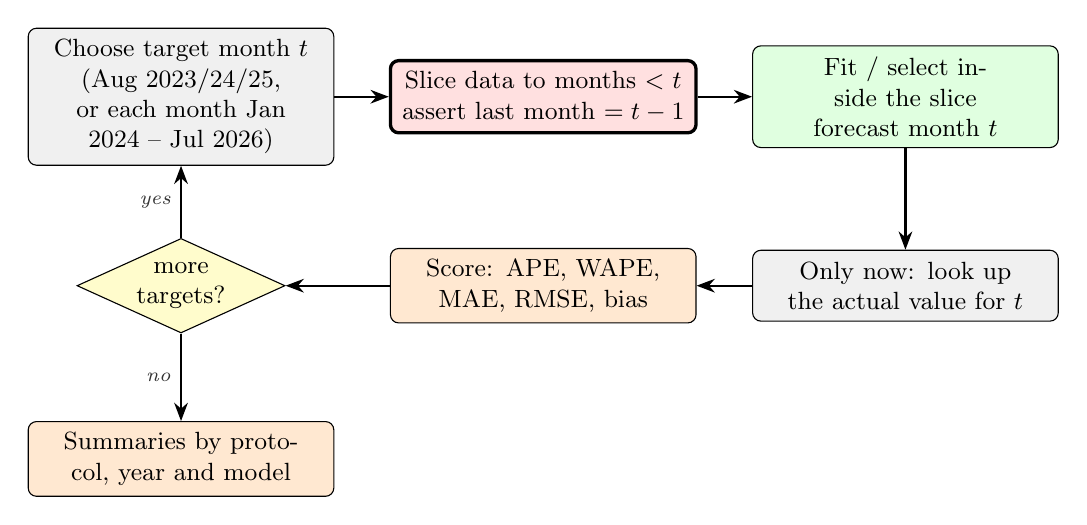
\begin{tikzpicture}
\node[proc=36mm] (pick) at (0,0) {Choose target month $t$\\ (Aug 2023/24/25, or each month Jan 2024 -- Jul 2026)};
\node[gate=36mm] (slice) at (4.6,0) {Slice data to months $< t$\\ assert last month $= t-1$};
\node[model=36mm] (fit) at (9.2,0) {Fit / select inside the slice\\ forecast month $t$};
\node[proc=36mm] (look) at (9.2,-2.4) {Only now: look up the actual value for $t$};
\node[out=36mm] (score) at (4.6,-2.4) {Score: APE, WAPE, MAE, RMSE, bias};
\node[dec] (more) at (0,-2.4) {more\\ targets?};
\draw[flow] (pick) -- (slice);
\draw[flow] (slice) -- (fit);
\draw[flow] (fit) -- (look);
\draw[flow] (look) -- (score);
\draw[flow] (score) -- (more);
\draw[flow] (more) -- node[left, lab]{yes} (pick);
\node[out=36mm] (sum) at (0,-4.6) {Summaries by protocol, year and model};
\draw[flow] (more) -- node[left, lab]{no} (sum);
\end{tikzpicture}
\caption{The backtest loop used in every stage. Protocol A: the three August folds.
Protocol B: 31 one-month-ahead origins.}\label{fig:loop}
\end{figure}

\noindent Any tuning a model needs (damping factor, window length, local-model choice, network
weights) happens inside the ``fit / select'' box, using only the slice. No parameter is tuned
against the backtest scores themselves.

\section{Inside the final model}
For August 2026 the final script repeats the same steps for each of the three outcomes (visits,
pounds, individuals) and each county.

\begin{figure}[H]\centering
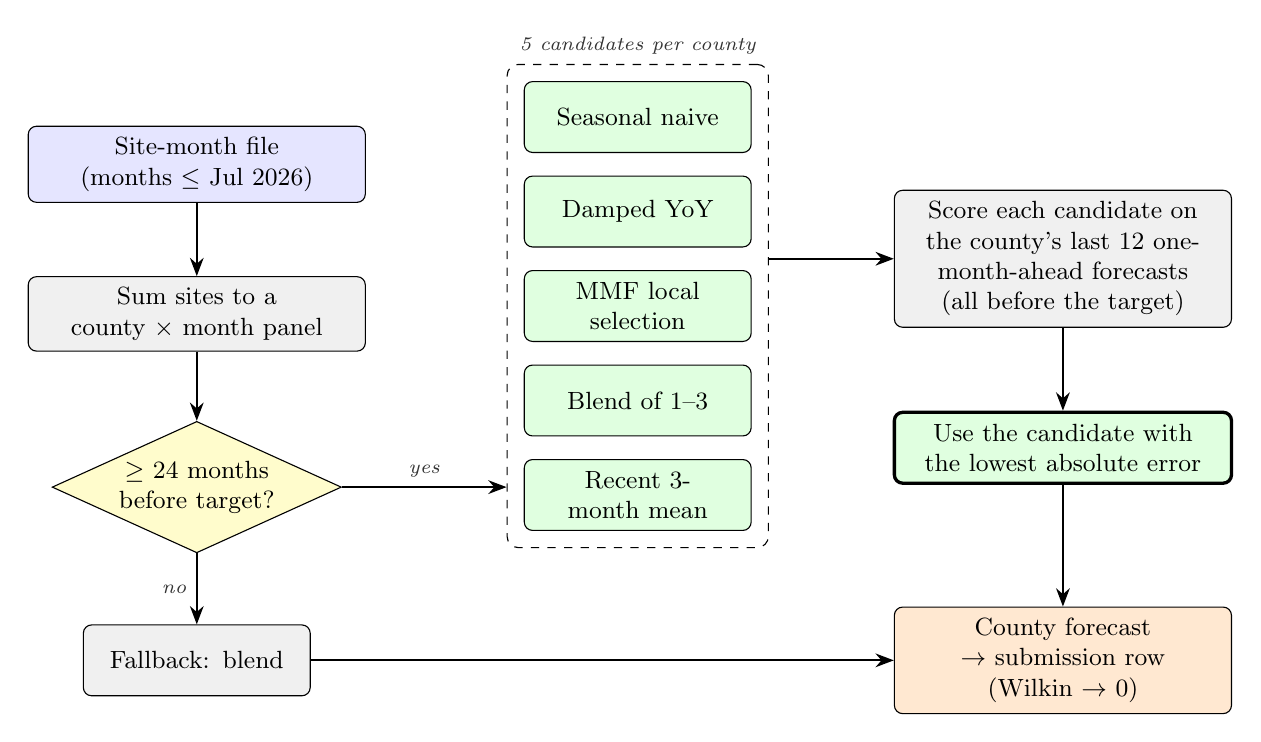
\begin{tikzpicture}
\node[data=40mm] (in) at (0,0) {Site-month file\\ (months $\le$ Jul 2026)};
\node[proc=40mm] (panel) at (0,-1.9) {Sum sites to a\\ county $\times$ month panel};
\node[dec] (hist) at (0,-4.1) {$\ge$ 24 months\\ before target?};
\node[model=26mm] (c1) at (5.6,0.6) {Seasonal naive};
\node[model=26mm] (c2) at (5.6,-0.6) {Damped YoY};
\node[model=26mm] (c3) at (5.6,-1.8) {MMF local selection};
\node[model=26mm] (c4) at (5.6,-3.0) {Blend of 1--3};
\node[model=26mm] (c5) at (5.6,-4.2) {Recent 3-month mean};
\begin{scope}[on background layer]
\node[draw, dashed, rounded corners, fit=(c1)(c5), inner sep=6pt, label={[lab]above:5 candidates per county}] (cands) {};
\end{scope}
\node[proc=40mm] (score) at (11.0,-1.2) {Score each candidate on the county's last 12 one-month-ahead forecasts (all before the target)};
\node[model=40mm, very thick] (pick) at (11.0,-3.6) {Use the candidate with the lowest absolute error};
\node[proc=26mm] (fb) at (0,-6.3) {Fallback: blend};
\node[out=40mm] (out) at (11.0,-6.3) {County forecast\\ $\rightarrow$ submission row\\ (Wilkin $\rightarrow$ 0)};
\draw[flow] (in) -- (panel);
\draw[flow] (panel) -- (hist);
\draw[flow] (hist.east) -- node[above, lab]{yes} (cands.west |- hist.east);
\draw[flow] (cands.east |- score.west) -- (score.west);
\draw[flow] (score) -- (pick);
\draw[flow] (pick) -- (out);
\draw[flow] (hist) -- node[left, lab]{no} (fb);
\draw[flow] (fb) -- (out);
\end{tikzpicture}
\caption{How the final model forecasts one county. Counties with a recent level shift (for example a
new site) tend to choose the recent mean; stable counties keep the blend or seasonal naive.}\label{fig:final}
\end{figure}

\begin{table}[H]\centering\small
\caption{The five candidates the final model chooses from, for a target month $t$.}\label{tab:cands}
\begin{tabularx}{\textwidth}{L{3.4cm}X}
\toprule
Candidate & Definition\\
\midrule
Seasonal naive & $\hat y_t = y_{t-12}$\\
Damped 3-month YoY & $\hat y_t = y_{t-12}\,\big(1 + 0.5\,(g-1)\big)$, where $g = \sum_{k=1}^{3} y_{t-k} \big/ \sum_{k=1}^{3} y_{t-12-k}$\\
MMF local selection & whichever of \{seasonal naive, damped YoY, full YoY, recent mean, recent level $\times$ last year's seasonal shape\} had the lowest error over the last 6 months\\
Blend & mean of the three candidates above\\
Recent 3-month mean & $\hat y_t = \tfrac13 \sum_{k=1}^{3} y_{t-k}$\\
\bottomrule
\end{tabularx}
\end{table}

\noindent For August 2026 the visits forecasts used the recent mean in 33 counties, damped YoY in 21,
the blend in 14, seasonal naive in 10, and MMF selection in 8.

\section{Where the cutoff is enforced}

\begin{table}[H]\centering\small
\caption{Cutoff checks and where they live.}\label{tab:cutoff}
\begin{tabularx}{\textwidth}{L{5.2cm}X}
\toprule
Check & Implementation\\
\midrule
No source month after July 2026 & \texttt{harness.load\_site}, \texttt{make\_submission.load\_site}: assertion on the maximum month\\
Training slice ends at $t-1$ & \texttt{harness.make\_context}, \texttt{make\_submission.county\_panel}: assertion on every call ($\sim$10{,}000 calls across the study)\\
Actuals looked up after forecasting & \texttt{harness.evaluate}, \texttt{make\_submission.backtest}: actual retrieved only after the forecast is stored\\
Selection uses only earlier origins & \texttt{make\_submission.county\_select}: the 12 scoring origins all lie before the target\\
External data lagged & \texttt{experiments/external\_predictors.py}: SNAP and calls only from at least 2--5 months before the target; the SNAP dashboard is truncated at July 2026\\
Audit trail & every run writes \texttt{cutoff\_check.txt}\\
\bottomrule
\end{tabularx}
\end{table}

\section{Folder layout and run order}

\begin{minipage}[t]{0.47\textwidth}\small
\textbf{Folder layout}
\begin{verbatim}
forecast_august_2026/
  README.md
  submission/          <- final model
    make_submission.py
    submission_template.csv
    Undergraduate_Predictions_Submit.csv
    county_backtest_*.csv
    statewide_forecast.csv
    cutoff_check.txt
  multiagent/          <- stages 1-2
    harness.py
    SELECTION_RULE.md
    combine.py
    honest_selection.py
    baselines/ stats/ panel_ml/
    deep_foundation/ structural/
  experiments/         <- stage 3
    county_tailoring.py
    external_predictors.py
    results/
  report/
    make_figures.py
    forecasting_report.tex/.pdf
    pipeline_flow.tex/.pdf
\end{verbatim}
\end{minipage}\hfill
\begin{minipage}[t]{0.5\textwidth}\small
\textbf{Run order} (from \texttt{forecast\_august\_2026/})
\begin{enumerate}[leftmargin=1.5em]
  \item \texttt{python multiagent/harness.py}\\ reference models ($\approx$2\,s)
  \item \texttt{python multiagent/<agent>/run.py}\\ optional; 2--20\,min each, results already saved
  \item \texttt{python multiagent/combine.py}\\ leaderboards and selection rule
  \item \texttt{python experiments/county\_tailoring.py}\\ chooses the final model
  \item \texttt{python experiments/external\_predictors.py}\\ SNAP and calls tests
  \item \texttt{python submission/make\_submission.py -{}-team-id ID}\\ final submission ($\approx$1\,min)
  \item \texttt{python report/make\_figures.py}\\ then compile the two \texttt{.tex} files
\end{enumerate}
\medskip
Only step 6 is needed to regenerate the submission; steps 1--5 reproduce the evidence behind it.
\end{minipage}

\section{Design decisions in one place}
\begin{itemize}
  \item \textbf{One data source, one gate.} The submitted model reads only the prepared site-month file,
        and every model goes through the same cutoff-checked slicing.
  \item \textbf{Same horizon everywhere.} All tests are one month ahead, matching the real task (July data
        $\rightarrow$ August forecast).
  \item \textbf{Two evaluation protocols.} Three August folds (the official question) plus 31 monthly
        origins (enough points to separate real gains from noise).
  \item \textbf{Simple components, adaptive selection.} Advanced models and external predictors were tested
        and rejected on out-of-sample evidence; the gain comes from letting each county choose among
        robust methods based on its own recent track record.
  \item \textbf{Everything reproducible.} Each table and figure has a script, and each run leaves a cutoff audit.
\end{itemize}

\end{document}
